\chapter{Identificação de múons}

Este capítulo descreve a elaboração de um modelo capaz de discriminar partículas
de múons com momento transverso elevado. O intuito é recuperar aquelas que
foram erroneamente classificadas no primeiro nível de filtragem como de baixa
energia por falharem ao cruzar as três camadas do RPC. 

A Seção~\ref{sec:data-section} apresenta os conjuntos de dados formados para a
realização das análises. Aa Seção~\ref{sec:performance_indexes} mostra os
índices de desempenho utilizados para avaliar os resultados obtidos. A seção
seguinte apresenta a metodologia utilizada.

\section{Apresentação das Bases de Dados}
\label{sec:data-section}

Os dados utilizados para realização das análises deste trabalho foram obtidos em
colisões observadas no ATLAS, em 2011, cuja energia total foi igual a 7~GeV e
luminosidade máxima igual a $10^{29}\text{cm}^2\text{s}^{-1}$.

Foram consideradas as informações relativas a geometria da célula D do TileCal
($\phi$ e $\eta$) e do MS ($\phi$ e $\eta$) para um evento de múon.  A energia
($E_\text{D}$) depositada pela passagem da partícula na célula do calorímetro também
foi levada em consideração. Como explicado anteriormente, estas informações
estão presentes no L1, porém, sem grande acurácia.  Contudo, na elaboração dos
modelos apresentados no decorrer desse capítulo, foram utilizados os valores
calculados na etapa \emph{offline} da reconstrução de eventos. Desta maneira,
garante-se a precisão dos dados utilizados.

Algumas considerações são importantes sobre a natureza dos dados utilizados:

\begin{itemize}

    \item O RPC cobre somente a região de $\eta < 1,05$. Assim, regiões do
    TileCal com pseudo-rapidez acima de 1 não são utilizadas no seu
    \emph{trigger} de múon.  Deste modo, apenas as células D0, D1, D2 e D3 foram
    utilizadas nesta pesquisa (ver Figura 2.10).

    \item Ao longo deste trabalho de pesquisa foi utilizado o casamento entre a
    geometria do TileCal e do RPC. Contudo, devido à diferença de granularidade
    entre as células D e as RoI do RPC, e também a curvatura em $\eta$ na
    trajetória do múon, o mapeamento entre célula D e RoI torna-se complexo. Uma
    simplificação possível é mapear cada célula D em um setor de \emph{trigger}
    do RPC. Esse mapeamento é robusto à variação de pseudo-rapidez, já que
    somente a posição da célula em $\phi$ é levado em consideração.

\end{itemize}

A Figura~\ref{fig:muonrates} mostra um gráfico relacionando a eficiência de
classificação do \emph{L1Muon} ao momento transverso do múon. O valor de $p_T$
calculado de maneira \emph{offline} (eixo $x$) é usado para validar a escolha
do sistema \emph{online}. O cálculo realizado pelos algoritmos \emph(offlines)
utiliza informações do sistema MDT, como foi explicado em capítulos anteriores.

\begin{figure}[ht!]
    \centering
    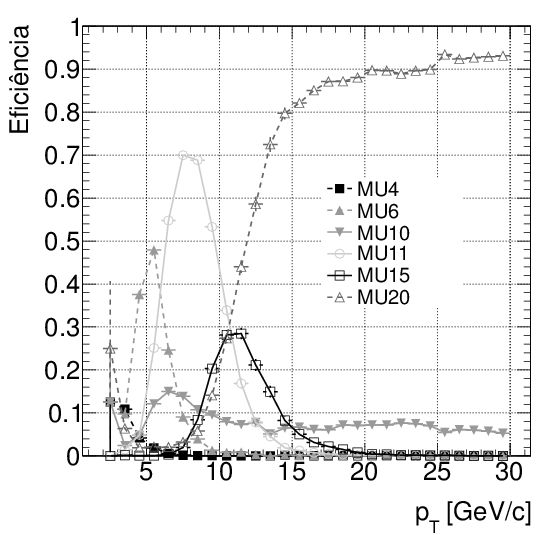
\includegraphics[width=12cm]{images/ppm_rpc_turnon_mu10.png}
    \caption{Eficiência de classificação do \emph{L1Muon} para eventos
    ocorridos no \emph{run} 191715.}
    \label{fig:muonrates}
\end{figure}

Pode-se observar que, como regra geral, a classificação obedece os patamares
preestabelecidos, ou seja, a distribuição de $p_T$ possui um pico em torno do
ponto de corte (por exemplo, 6~GeV para MU6) e final da calda antes do corte do
patamar seguinte. A única exceção é exatamente os eventos marcados como MU10,
cuja distribuição se prolonga até valores bastante elevados. Esse fato pode ser
explicado pelas áreas descobertas pelo terceiro plano RPC, por falhas no sistema
de alimentação do MS ou mesmo por múons que, mesmo com momento transverso
elevado, não conseguiram vencer o campo magnético toroidal.

Esse trabalho visa recuperar esses múons que foram classificados de maneira
equivocada. Para tal, foram projetados dois classificadores com objetivo
distintos com bases próprias:

\begin{enumerate}
    \item Classificador capaz de identificar se partículas marcadas como MU10 são
    realmente limitadas pelo patamar inferior de 10~GeV. Para esta análise, foram
    utilizados dados do \emph{run} 191715. São eventos datados de outubro de 2011. A
    configuração do detector previa a aquisição de múons independentes (eventos do
    tipo \emph{single muon} ou simplesmente \emph{sglmuon}). Eventos com $p_T >
    10$~GeV (totalizando 3518) são estudados enquanto os restantes (365) são
    considerados falsos-alarmes.

    \item A etapa de  \emph{offline} classifica múons através de três critérios
    que variam de acordo com a acurácia desejada: \emph{tight}, \emph{medium} e
    \emph{loose}. O classificador projetado usou como alvo eventos aprovados
    pelo critério \emph{tight}. Eventos qualificados apenas no critério
    \emph{loose} foram considerados falsos-alarmes.  Neste projeto, foram
    utilizados dados de todos os \emph{2011} que foram configurados como
    \emph{minbias}. Nesta configuração, múons não são o principal objetivos,
    sendo assim, ruído de fundo do experimento. Usou-se essa configuração com
    intuito de isolar os efeitos do L1 em  relação ao classificador. Foram 2252
    eventos alvo contra
    430 indesejados.

\end{enumerate}

A Tabela~\ref{table:Classes} resume o número de eventos e a configuração
utilizada

\begin{table}[htbp!]
  \centering
  \begin{tabular}{ l  r  r  r  }
      \toprule
                         & Classe & Não-Classe & Configuração\\
      \midrule
        1 & 3518  & 365 & \emph{sglmuon} \\
        2 & 2252 & 430 &  \emph{minbias} \\ 
      \bottomrule
  \end{tabular}
  \caption{Resumo dos eventos MU10 considerados.}
  \label{table:Classes}

\end{table}



\section{Parâmetros de Avaliação do Desempenho}
\label{sec:performance_indexes}
A avaliação de eficiência dos algoritmos propostos nesse trabalho é realizada
através da utilização da curva ROC (\emph{Receiver Operating
Characteristic})~\cite{TREES2001} e pelo índice SP~\cite{ref:SIMAS}.

A curva ROC mostra como as probabilidades de detecção e falso alarme variam com
o patamar de decisão. A eficiência de um classificador pode ser estimada a
partir da área sob a curva ROC. Quanto maior a área, mais eficiente é o
discriminador~\cite{ref:SIMAS}.

O índice SP é definido por~\cite{CIODARO2012}:

\begin{equation}
SP = \sqrt{\sqrt{P_{\text{c}}P_{\text{nc}}} \left(\frac{P_{\text{c}} +
P_{\text{nc}}}{2}\right)}
\end{equation}

onde $P_\text{c}$ é a probabilidade de detecção da classe desejada e
$P_{\text{nc}}$ é a probabilidade de não obter um falso alarme.

O SP é  o parâmetro para escolher o patamar de decisão ótimo para um
classificador~\cite{ref:SIMAS}. Variando-se o patamar de decisão em toda sua
faixa de excursão, calculam-se os valores do SP correspondentes. O SP máximo
indica um patamar que apresenta alta eficiência para as duas classes.

\section{Metodologia}

Esta Seção apresenta a metodologia utilizada na tentativa de alcançar os
objetivos traçados anteriormente. Três abordagens foram realizadas: estudo da
deposição de energia de uma partícula passante na célula D do TileCal; utilizar
a geometria do detector ATLAS como fator classificatório; projeto de
discriminadores neurais utilizando os parâmetros disponíveis no L1, confirmados
pela reconstrução \emph{offline} de múons.

\subsection*{Deposição de Energia}

Nesta abordagem, o histograma de distribuição da energia depositada pela
passagem de múons na camada externa do calorímetro hadrônico foi comparado com o
conjunto de falsos alarmes de cada um dos grupos descritos na
Seção~\ref{sec:data-section}.

Sabe-se que o ruído de fundo captado pelas células D possui média igual à 150
MeV e que a relação sinal-ruído é relativamente baixa, o que dificulta a
utilização de patamares de energia~\cite{CIODARO2009}. Porém, há a possibilidade
de definir um patamar, acima do nível de ruído, capaz de aumentar a eficiência
de detecção, sem comprometer a taxa de eventos estabelecida para o L1, ou seja,
sem aumentar substancialmente a quantidade de falsos alarmes.

\subsection*{Casamento de Geometria}

Outra possibilidade é a utilização da geometria do calorímetro hadrônico e do
RPC. Como explicado, múons são elementos pesados e, portanto, sofrem pouca ação
dos campo magnéticos que atuam no ATLAS. Contudo, múons menos energéticos tendem
a ser desviados de modo mais acentuado. Ao dividir o ATLAS em setores azimutais
(setores de \emph{trigger}), em torno do ponto de interação, é possível
identificar quais partículas possuem trajetórias mais oblíquas.

O RPC é dividido logicamente em ROI, que são agrupadas em
setores de trigger. A informação de cada um desses setores, por sua vez, é
controlada por uma Sector Logic~(SL). Não há, porém, uma relação direta entra
as células D do calorímetro e uma RoI, devido a diferença de granularidade.
Entretanto, um casamento entre o módulo do TileCal e o setor de trigger
correspondente é viável. Deste modo, todas as células D do detector são
mapeadas nos setores de
\emph{trigger} do MS, de acordo com as suas posições $\phi$.

Nesta abordagem só são considerados múons de interesse os que cruzam um setor de
\emph{trigger}, quando combinadas com as informações geométricas da célula D.



\subsection*{Discriminador Neural}

As redes neurais artificiais~(RNA)~\cite{WASSERMAN1989,HAYKIN2008} são modelos
matemáticos inspirados em algumas características do cérebro humano, sendo
capazes de adquirir conhecimento e generalizar. Devido ao poder computacional,
obtido de sua estrutura paralelamente distribuído e suas habilidades, as RNAs
são usadas em diversas aplicações: reconhecimento de padrões~\cite{BISHOP1995},
controle e identificação de sistemas~\cite{ICHIKAWA1992}, processamento de
sinais~\cite{LAPEDES1987}, aproximação de funções~\cite{DENG2011}.

Uma diferença fundamental entre os classificadores neurais e os métodos
clássicos é que nestes últimos é necessário formular um modelo matemático a
partir dos sinais. Na abordagem neural, o classificador trabalha diretamente no
conjunto de dados, ficando o modelo matemático implícito nos valores dos pesos
sinápticos obtidos após o treinamento~\cite{ref:SIMAS}.

As redes de múltiplas camadas \emph{feed-forward} são compostas a partir da
formação sequencial de duas ou mais camadas de neurônios. A rede é composta por
três camadas: a entrada, a camada oculta e a saída. A camada oculta é
responsável por extrair características estatísticas de ordem elevada. Neste
trabalho foram utilizados sete neurônios na entrada e apenas um na saída. A
quantidade de neurônios da camada intermediária foi determinada mediante estudo
apresentado nas seções seguintes. A saída da rede foi projetada para resultar
$-1$ para eventos não desejados e $1$ para detecção. A Figura~\ref{fig:nnArch}
apresenta o modelo genérico de redes utilizados neste trabalho.

\begin{figure}[htbp!]
    \centering
    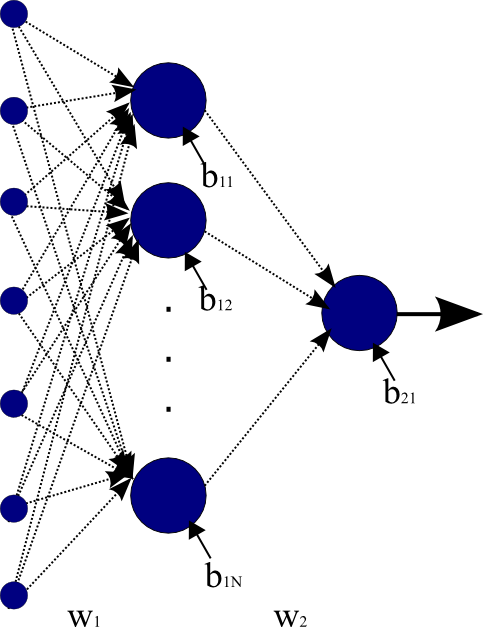
\includegraphics[height=6.5cm]{images/nnschema.png}
    \caption{Modelo de redes neurais utilizadas para discriminar os sinais de
    múons.}
    \label{fig:nnArch}
\end{figure}

As seguintes etapas foram realizadas para o projeto do discriminador neural.

\subsubsection{Robustez à Extrapolação em $\phi$ ($\phi$ \emph{Wrap-Around})}

As variáveis $\phi_\text{D}$ e $\phi_{\text{RoIRPC}}$ têm característica circular
e estão definidas no intervalo fechado ($-\pi$, $+\pi$). É possível ocorrerem
eventos onde, por exemplo, $\phi_\text{D}$ encontra-se próxima ao plano $\phi =
-\pi$ e a variável $\phi_{\text{RoIRPC}}$ esteja localizada no extremo oposto.
Para evitar esta distorção e manter a característica das variáveis em questão,
as seguintes transformações foram aplicadas:

\begin{eqnarray}
p^1 = \sin(\phi)\\
p^2 = \cos(\phi)
\end{eqnarray}

Deste modo, as variáveis $p^1_\text{D}$, $p^1_\text{RoIRPC}$, $p^2_\text{D}$,
$p^2_\text{RoIRPC}$ passam a ser utilizadas no treinamento, validação e operação
das redes neurais.

\subsubsection{Pré-processamento}

Para normalização a entrada e alvos da rede foram utilizadas a média e o desvio
padrão do conjunto de treino. Desta maneira, objetiva-se retirar a componente
média da amostra e deixar o desvio padrão unitário. Após o treinamento da rede,
os valores usados nesta normalização passam a fazer parte da rede, tanto quanto
as sinapses, devendo ser aplicados posteriormente no conjunto de teste e
validação.


\subsubsection{Especificação da Topologia}

Para decidir a quantidade de neurônios presentes na camada oculta, optou-se por
realizar uma série de treinos para 30 arquiteturas diferentes. Cada neurônio,
em todas as arquiteturas utilizadas, empregou a tangente hiperbólica como
função de ativação. A topologia que apresentar o maior valor médio para o índice
SP, considerando todas as rodadas utilizadas, foi considerada a melhor rede.

\subsubsection{Treinamento}

Os conjuntos utilizados foram separados de tal forma que 70\% dos eventos de
cada classe foram empregados para o desenvolvimento do pré-processamento e
treinamento. Mais 20\% foram separados para a análise do critério de
parada das redes empregadas. O restante serve para a validação pós-treino. Esse
procedimento será explicado mais adiante.

Os pesos foram inicializados utilizando valores aleatórios entre -0,2 e 0,2. O
treinamento utilizado foi o algoritmo \emph{Resilient
Backpropagation}~\cite{RIEDMILLER1993}. Ao final do treinamento, a rede neural
guardou as sinapses que proporcionaram o menor valor de MSE, de acordo com o
critério \emph{Save the Best}.

A Tabela~\ref{table:nnparameters} apresenta os valores utilizados para cada
parâmetro de treinamento.


\begin{table}[htbp!]\footnotesize
  \centering
  \tabcolsep=0.08cm
  \begin{tabular}{ m{7cm} m{3cm} }
      Parâmetro & Valor \\
      \midrule
      Figura de mérito           & MSE mínimo \\
      Número máximo de épocas    & 200.000 \\
      Gradiente mínimo           & $1e-10$ \\
      Taxa de aprendizagem       & 0.01 \\
      Mudança máxima de peso sinápticos    & 50\% \\
      Número máximo de falhas    & 1000 \\
      Número de inicializações   & 20 \\
      \bottomrule
  \end{tabular}
  \caption{Valores utilizados para cada parâmetro do treinamento neural.}
  \label{table:nnparameters}

\end{table}

\subsubsection{Análise da Flutuação Estatística}

Para que a flutuação estatística inerente aos dados empregados possa ser levada
em consideração na composição dos resultados, todos os discriminadores
desenvolvidos foram analisados através da validação cruzada~\cite{HAYKIN2008}.
Aqui, a validação foi realizada respeitando as seguintes etapas.

\begin{enumerate}
    \item Divide-se todo o conjunto em \emph{clusters} utilizando o algoritmo de
    \emph{K-Means}~\cite{HARTIGAN1979}. O número de agrupamentos é definido pelo
    índice de Davies--Bouldin~\cite{DAVIES1979}.
    \item Distribuem-se os \emph{clusters} igualmente entre 10 blocos. Desta
    maneira, espera-se que cada bloco possua características estatísticas
    similares entre si. Além disso, cada bloco constitui uma representação em
    menor escala do conjunto todo.
    \item Sete blocos são separados para o conjunto, dois blocos para validação
    e um para teste.
    \item O discriminador neural é treinado.
    \item Os resultados obtidos são armazenados
    \item Os últimos três passos são então repetidos nove vezes variando a
    seleção de blocos, e nunca repetindo aquele já selecionado para o conjunto
    de teste em um treinamento anterior para a mesma função.
\end{enumerate}


%%%%%%%%%%%%%%%%%
%%%
%%% Resultados
%%%%%%%%%%%%%%%%%%

\chapter{Resultados e Discussão}

Neste capítulo, são apresentados os resultados obtidos ao aplicar a metodologia
indicada no capítulo anterior. Os dados utilizados foram obtidos em colisões
observadas no ATLAS, em 2011, cuja energia total foi igual a 7~GeV.

Foram utilizadas as informações relativas a geometria da célula D do TileCal
($\phi$ e $\eta$) e do MS ($\phi$ e $\eta$) para um evento de múon.  A energia
($E_\text{D}$) depositada pela passagem da partícula na célula do calorímetro também
foi levada em consideração.

Foram projetados dois classificadores com objetivos distintos com bases
próprias. O primeiro é capaz de identificar se partículas marcadas como MU10
são realmente limitadas pelo patamar inferior de 10~GeV. Para esta análise,
foram utilizados dados do \emph{run} 191715. O segundo usou como alvo eventos
aprovados pelo critério \emph{tight}. Eventos qualificados apenas no critério
\emph{loose} foram considerados falsos-alarmes.  Aqui, foram utilizados dados
de todos os  \emph{runs} de 2011 que foram configurados como \emph{minbias}.


\section{Discriminação de múons de alto $p_T$ e baixo $p_T$}

Existe uma região de confusão entre múons de alto e de baixo momento
transverso, em torno de 10~GeV. Essa característica faz com que uma parte dos
múons de alto momento transverso sejam sempre identificados pelo patamar MU10,
sensível aos múons de baixo $p_T$. Assim, esse patamar opera com um elevado
prescale, o que diminui a quantidade de múons de alto momento transverso
observados.

Nesta etapa, procurou-se verificar se a célula D serviria como substituta da
camada do RPC faltante. Uma terceira etapa de coincidência deixa a aquisição
menos sensível a múons de baixo $p_T$, aumentando a a probabilidade de detectar
múons de alta energia corretamente.


\subsection*{Deposição de Energia}

O histograma da distribuição de energia depositada pela passagem de múons de
alto $p_T$ na célula D foi comparado com o conjunto de múons de baixo $p_T$.
Todos foram classificados no \emph{online} como MU10, e seus respectivos
momentos foram estimados pelo \emph{offline}. Na
Figura~\ref{fig:histEnergy191715}, pode-se verificar que as duas distribuições
são muito similares, o que dificulta a determinação de um patamar que possa ser
aplicado aos sinais e atue como um discriminador. Outro detalhe visível é  a
distância das duas distribuições em relação ao ruído eletrônico (ou
\emph{pedestal}).

\begin{figure}[htpb!]
    \centering
    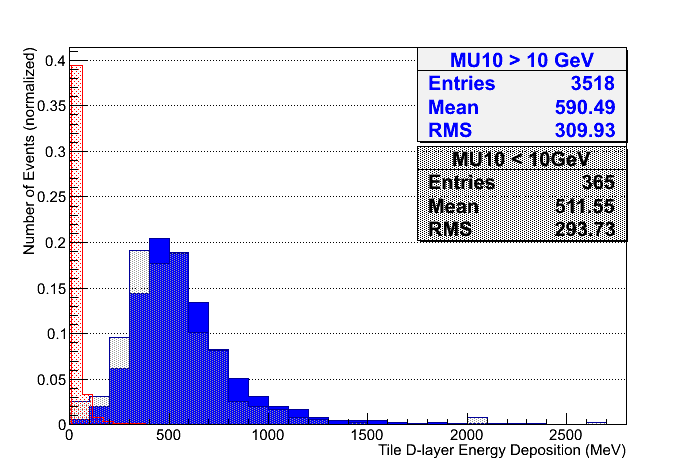
\includegraphics[width=10cm]{images/sglmuon/histEnergyDeposition.png}
    \caption{Distribuição da energia depositada na célula D do TileCal durante o
    \emph{run} 191715. Em azul, os múons com $p_T >$ 10~GeV. Em cinza, os múons
    com $p_T <$ 10~GeV. Em vermelho, a distribuição do ruído eletrônico.}
    \label{fig:histEnergy191715}
\end{figure}

Como pode-se observar na Figura~\ref{fig:ROCEnergy191715}, a eficiência de
detecção para as duas classes é muito semelhante. A curvatura da curva ROC é
muito sutil. O ponto de SP máximo dá-se quando o patamar de corte é igual a
500~MeV, onde a taxa detecção chega a aproximadamente 60\% e o falso-alarme
fica acima de 50\%.

Percebe-se assim que um corte por patamar de energia sozinho não é suficiente
para distinguir a classe alvo.

\begin{figure}[H]
        \centering
        \begin{subfigure}[b]{0.45\textwidth}
                \centering
                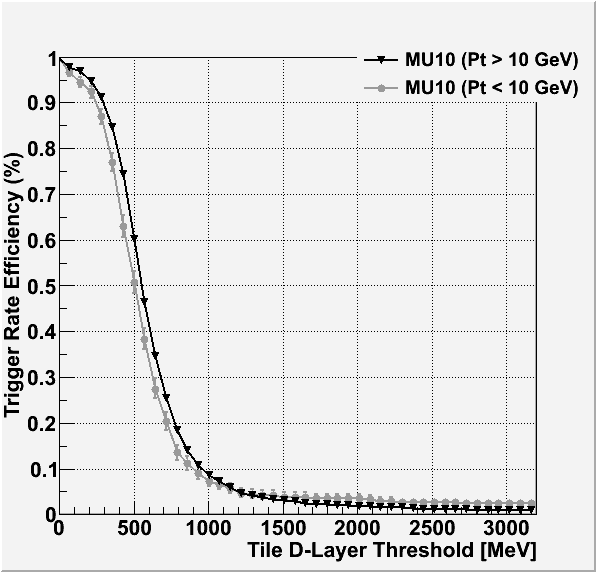
\includegraphics[width=\textwidth]{images/sglmuon/roc_nomatch.png}
        \end{subfigure}%
        ~
        \begin{subfigure}[b]{0.45\textwidth}
                \centering
                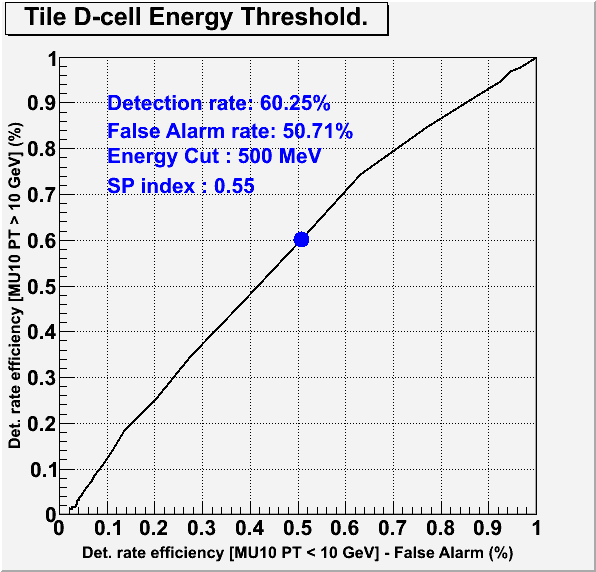
\includegraphics[width=\textwidth]{images/sglmuon/roc_perf_nomatch.png}
        \end{subfigure}
        \caption{Curva ROC para o uso de patamar de energia.}
        \label{fig:ROCEnergy191715}
\end{figure}



\subsection*{Casamento de Geometria}

A Figura~\ref{crossgeo} procura mostrar o quão oblíquo é a trajetória dos múons
que cruzaram o TileCal e o RPC durante o \emph{run} escolhido. No eixo $x$,
encontramos a diferença em $\eta$ entre os pontos de cruzamentos na célula D e
no RoI do RPC. A escala de cor representa a quantidade de eventos que obtiveram
a mesma inclinação. O histograma superior apresenta os eventos com baixo $p_T$ e
o inferior com alto $p_T$. Pode-se notar que a distribuição do primeiro é mais
dispersa, principalmente em $\phi$. Este comportamento deve-se ao fato de múons
menos energéticos tendem a ser desviados de modo mais acentuado.

\begin{figure}[htpb!]
    \centering
    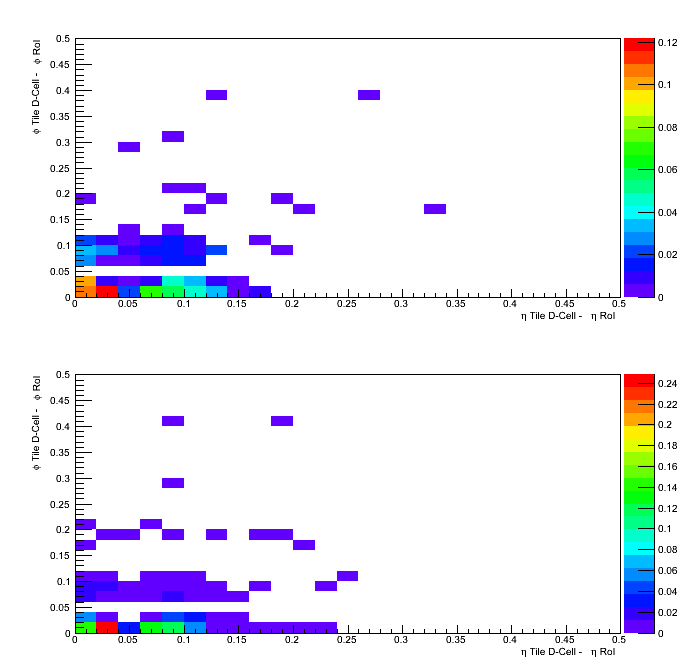
\includegraphics[width=11cm]{images/sglmuon/crossGeo.png}
    \caption{Histograma apresentando o quão oblíqua é a trajetória do múon. O
    primeiro gráfico representa os eventos com partículas com baixo momento
    transverso e o segundo com alto.}
    \label{crossgeo}
\end{figure}

É estabelecer um novo patamar de corte ao rejeitar todas as partículas que
atravessem  setores de \emph{trigger} distintos. Para tal, as células D do
detector são mapeadas, de acordo com as suas posições $\phi$, em relação aos
setores do espectrômetro.

A partir da Figura~\ref{fig:ROCSL191715} conclui-se que, apesar de excluir
partículas também do conjunto alvo, casando as geometrias dos dois detectores há
uma melhora na taxa de detecção. A curva ROC possui um ângulo de inclinação mais
acentuado em relação à curva apresentada anteriormente. O corte em energia passa
a ser aproximadamente 430~MeV. Desta forma, observa-se que considerar as
características geométricas do detector é interessante para a classificação.

\begin{figure}[htpb!]
        \centering
        \begin{subfigure}[b]{0.45\textwidth}
                \centering
                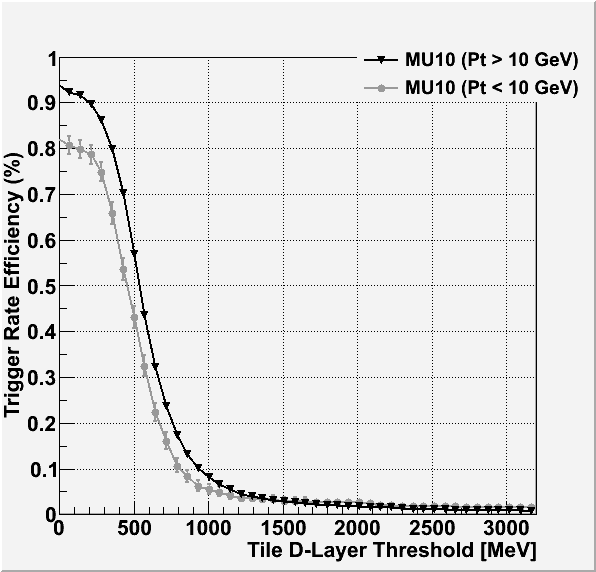
\includegraphics[width=\textwidth]{images/sglmuon/roc_match_SL.png}
        \end{subfigure}%
        ~
        \begin{subfigure}[b]{0.45\textwidth}
                \centering
                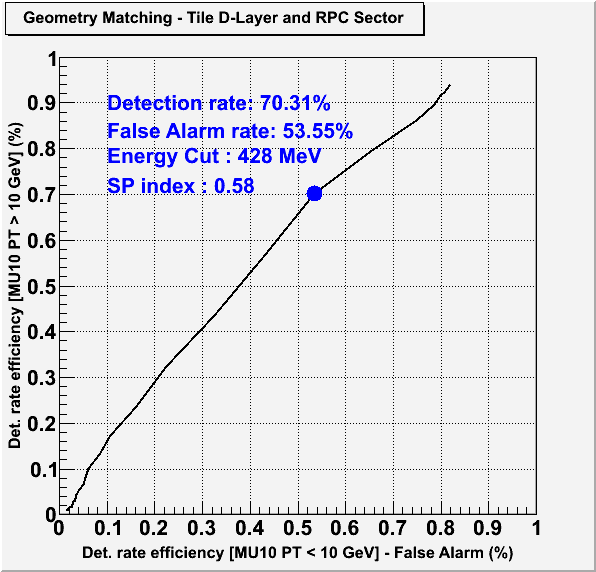
\includegraphics[width=\textwidth]{images/sglmuon/roc_perf_match_SL.png}
        \end{subfigure}
        \caption{Curva ROC para o uso de patamar de energia ao casar as
        geometrias do TileCal e do RPC.}
        \label{fig:ROCSL191715}
\end{figure}


\subsection*{Discriminador Neural}

A primeira etapa no projeto do discriminador neural foi separar os dados em
conjuntos de treino, teste e validação. Para a realização dos treinos, foi
escolhida como metodologia a validação cruzada, a fim de minimizar os efeitos da
flutuação estatísticas. Com ela, espera-se a obtenção de uma topologia ótima
para o problema.

Primeiramente, agrupou-se as amostras para evidenciar eventos com
características estatísticas semelhantes. O índice de Davies-Bouldin determinou
22 \emph{clusters} como ideal para o conjunto apresentado. O algoritmo
\emph{K-Means} foi utilizado para a tarefa. A Figura~\ref{fig:clusters191715}
mostra o resultado da divisão em agrupamentos. Interessante perceber que nenhum
dos \emph{clusters} formados evidenciou uma das classes.

\begin{figure}[htpb!]
    \centering
    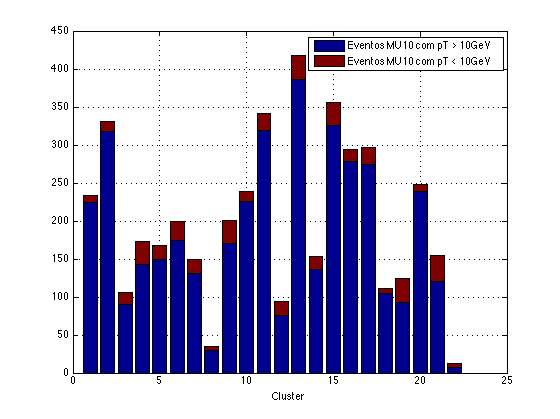
\includegraphics[width=11cm]{images/sglmuon/distribuicao_clusters.png}
    \caption{Eventos de múon separados em 22 \emph{clusters} depois de aplicado
    o algoritmo de \emph{K-means}. Em vermelho, estão representados os múons de
    baixo $p_T$. Em azul, os múons de alto $p_T$.}
    \label{fig:clusters191715}
\end{figure}

Os dados dos \emph{clusters} foram igualmente distribuídos entre 10 os blocos.
Desta maneira, espera-se que cada bloco possua características estatísticas
similares entre si.  As Figuras~\ref{fig:bloco191715-1}, \ref{fig:bloco191715-2} e
\ref{fig:bloco191715-3} mostram os dados distribuídos nos blocos. Neste ponto,
as informações sobre múons de baixo $p_T$ são replicadas em cada um dos blocos,
de forma que a representatividade das duas classes seja parelha.


\begin{sidewaysfigure}
    \centering
    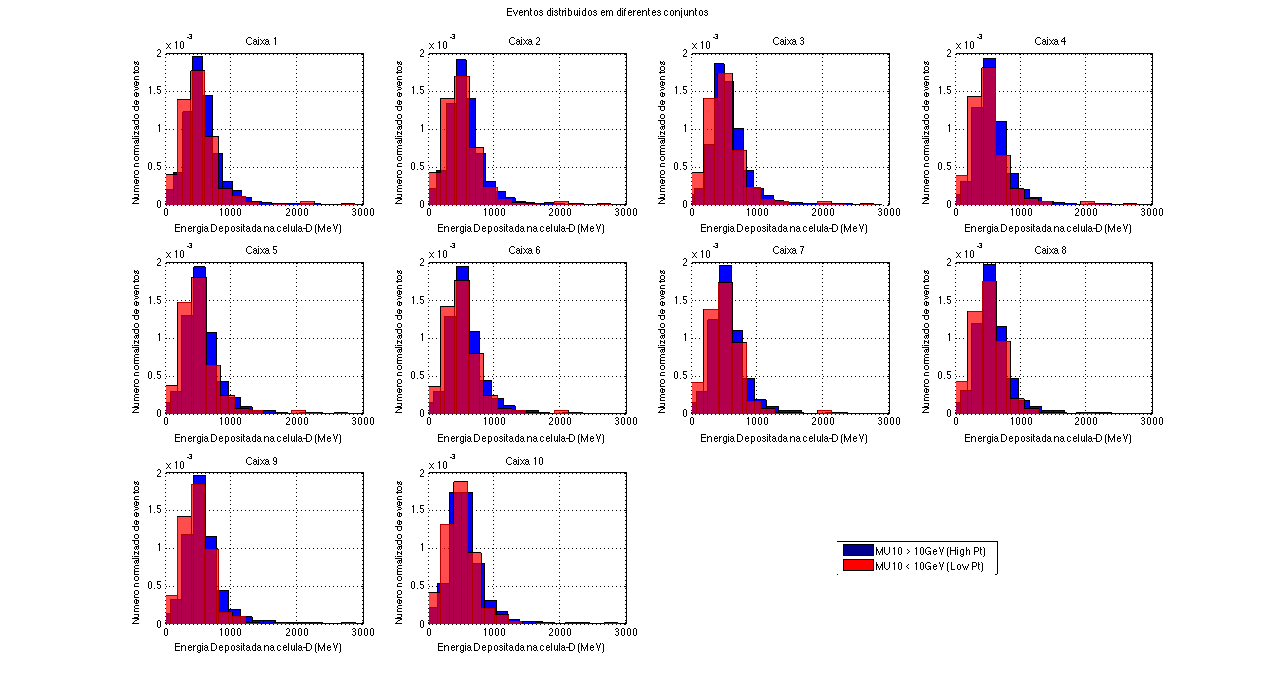
\includegraphics[width=\textheight]{images/sglmuon/eventos_caixas.png}
    \caption{Eventos de múons divididos em 10 blocos. As distribuições da
    energia depositada na célula D. Os histogramas dos diferentes blocos devem
    ser semelhantes.}
    \label{fig:bloco191715-1}
\end{sidewaysfigure}

\begin{sidewaysfigure}
    \centering
    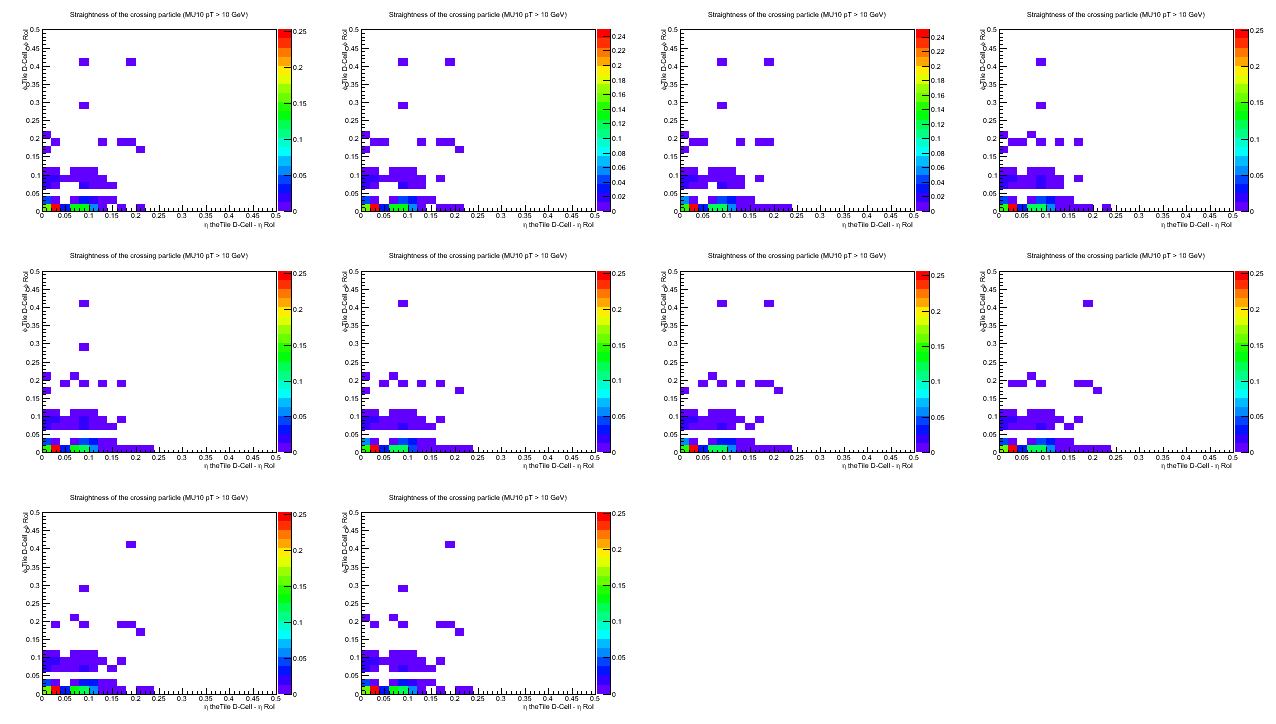
\includegraphics[width=\textheight]{images/sglmuon/cluster_eta_phi_class.png}
    \caption{Eventos de múons divididos em 10 blocos. \emph{Hits} na camada D do
    TileCal e nas regiões de interesse do RPC. Aqui estão representados os
    eventos de alto $p_T$}
    \label{fig:bloco191715-2}
\end{sidewaysfigure}

\begin{sidewaysfigure}
    \centering
    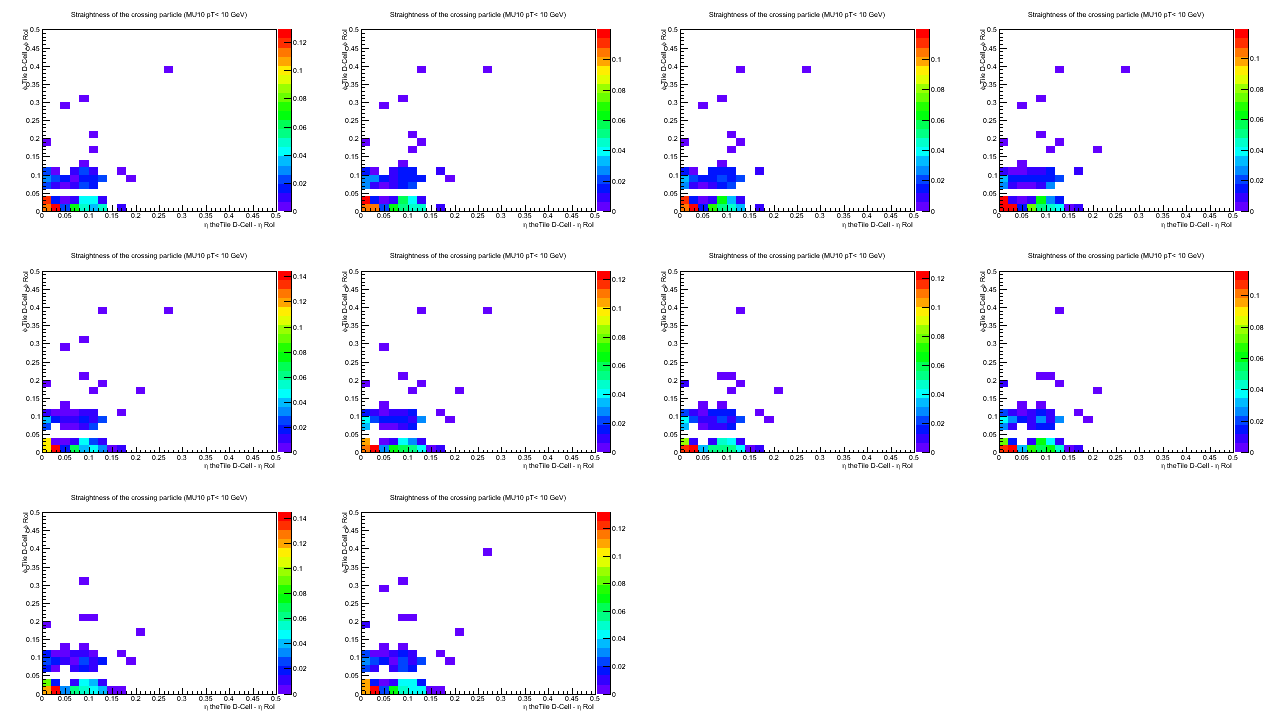
\includegraphics[width=\textheight]{images/sglmuon/cluster_eta_phi_noclass.png}
    \caption{Eventos de múons divididos em 10 blocos. \emph{Hits} na camada D do
    TileCal e nas regiões de interesse do RPC. Aqui estão representados os
    eventos de baixo $p_T$}
    \label{fig:bloco191715-3}
\end{sidewaysfigure}

Ao todo, 31 topologias foram treinadas. Por sua vez, cada uma foi treinada com
10 arranjos diferentes de treino, teste e validação. Cada rede foi inicializada
20 vezes com intuito de evitar mínimos locais e a que tiver melhor índice de SP
para o conjunto de validação será armazenada. No total, foram realizadas 6.200
rodadas de treino para selecionar a topologia ideal. 

A Figura~\ref{fig:Topology191715} mostra o índice de SP médio para cada
topologia treinada, levando em consideração os 10 blocos utilizados. No gráfico,
ainda é possível verificar o valor máximo e mínimo conseguido. A incerteza é
representada pelo desvio padrão. Levando em consideração o SP mais elevado, a
rede com 15 neurônios na camada escondida foi escolhida.

A Figura~\ref{fig:ROCNN191715} apresenta a  curva ROC para a rede com 15
neurônios na camada intermediária que obteve maior valor de SP. Observa-se que
ela obteve um ganho de 5\% em detecção em relação à proposta de casamento de
geometria.  Referente à taxa de falso-alarme, a rede proporcionou um grande
ganho, reduzindo-o para aproximadamente 15\%.


\begin{figure}[htpb!]
    \centering
        \begin{subfigure}[b]{0.45\textwidth}
                \centering
            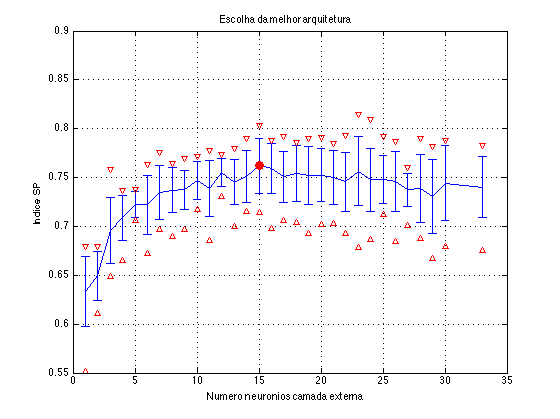
\includegraphics[width=\textwidth]{images/sglmuon/plotSP.png}
            \caption{Escolha da melhor Topologia. Com base nesse gráfico podemos
            perceber que a topologia com 15 neurônios obteve melhor desempenho.}
            \label{fig:Topology191715}
        \end{subfigure}%
        ~
        \begin{subfigure}[b]{0.45\textwidth}
                \centering
                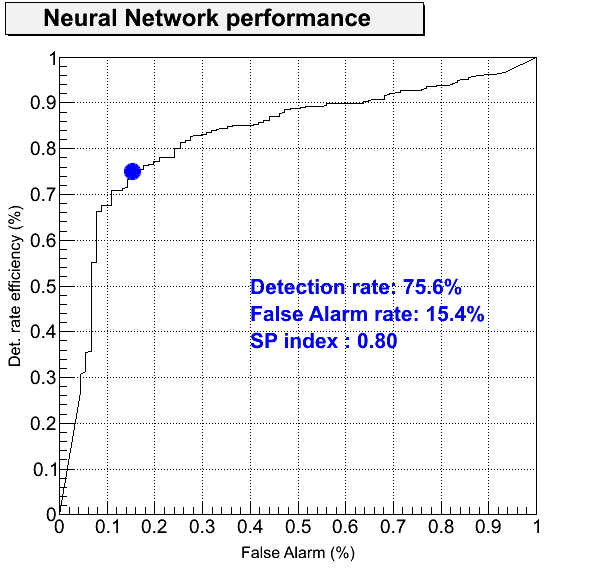
\includegraphics[width=\textwidth]{images/sglmuon/roc_perf_match_NN.png}
            \caption{Curva ROC para saída da rede neural com 15 neurônios na
            camada escondida.}
            \label{fig:ROCNN191715}
        \end{subfigure}
        \caption{Projeto de discriminador neural.}
\end{figure}

\section{Discriminação de múons verdadeiros e falsos.}

Como podemos notar pela Figura~\ref{fig:rejected} existe um grande número de
múons que são detectados pelo L1, mas posteriormente descartados pelos
algoritmos \emph{offline}.


\begin{figure}[htp!]
   \centering
   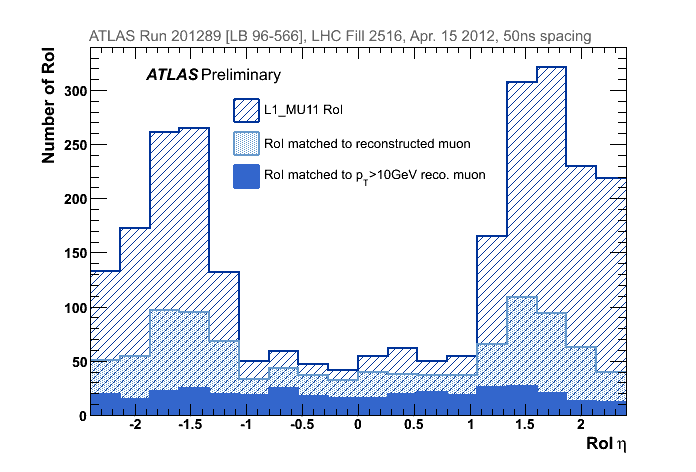
\includegraphics[width=11cm]{images/muon_rejected.png}
   \caption[Distribuição de RoI em $\eta$ com múons aprovados. É mostrado qual
   percentual é confirmado posteriormente pelos algoritmos \emph{offline} ]%
   {Distribuição de RoI em $\eta$ com múons aprovados. É mostrado qual
   percentual é confirmado posteriormente pelos algoritmos \emph{offline}
   (Retirado de~\cite{BUTTINGER2012}).}
   \label{fig:rejected}
\end{figure}
%%%

Nesta etapa, procurou-se verificar se a informação da  célula D ajudaria a
identificar falsos múons e assim, melhorar a eficiência do sistema de aquisição.


\subsection*{Deposição de Energia}


O histograma da distribuição de energia depositada pela passagem de múons
(partículas aprovadas pelo critério \emph{tight}) na célula D foi comparado com
o conjunto de falsos múons (rejeitados pelo \emph{tight}, mas, no caso,
aprovados pelo \emph{loose}).  Todos foram classificados no \emph{online} como
MU10, e seus respectivos momentos foram estimados pelo \emph{offline}. Na
Figura~\ref{fig:histEnergyminbias}, pode-se verificar que, como no caso
anterior,  as duas distribuições são muito similares.


\begin{figure}[htpb!]
    \centering
    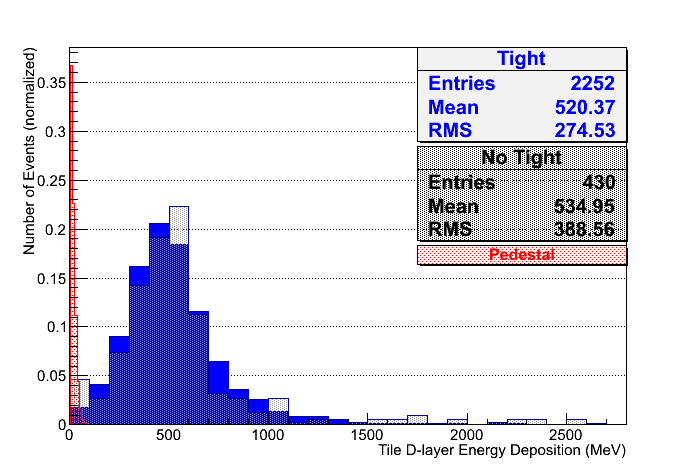
\includegraphics[width=12cm]{images/minbias/histEnergyDeposition.png}
    \caption{Distribuição da energia depositada na célula D do TileCal para
    todos os \emph{runs} de 2011 com configuração de \emph{minbias}.}
    \label{fig:histEnergyminbias}
\end{figure}


Como pode-se observar na Figura~\ref{fig:ROCEnergyminbias}, a eficiência de
detecção para as duas classes é muito semelhante. O coeficiente linear da curva
é unitário, ou seja, apenas a informação de energia é insuficiente para tarefa.
O ponto de SP máximo dá-se quando o patamar de corte é igual a 567~MeV, onde a
taxa detecção e o falso-alarme possuem taxas  aproximadamente 62\%.

\begin{figure}[htpb!]
        \centering
        \begin{subfigure}[b]{0.45\textwidth}
                \centering
                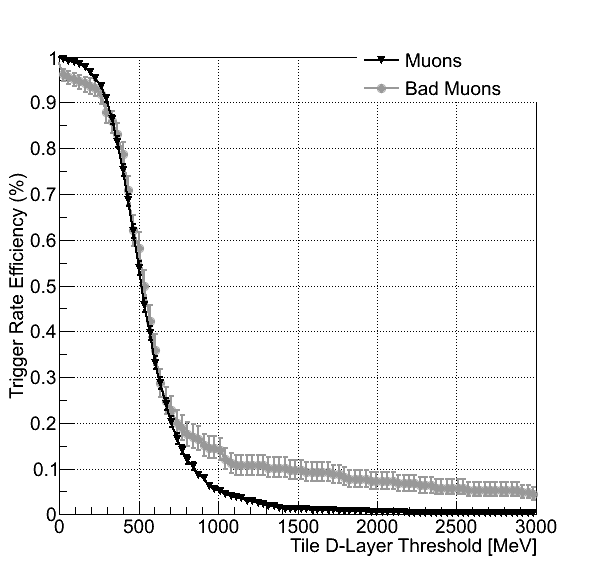
\includegraphics[width=\textwidth]{images/minbias/C.png}
        \end{subfigure}%
        ~
        \begin{subfigure}[b]{0.45\textwidth}
                \centering
                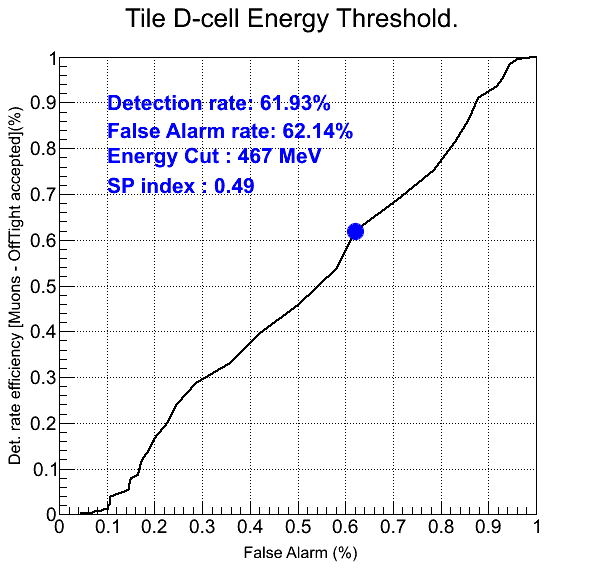
\includegraphics[width=\textwidth]{images/minbias/C_roc.png}
        \end{subfigure}
        \caption{Curva ROC ao considerar patamares de energia}
        \label{fig:ROCEnergyminbias}
\end{figure}G

\subsection*{Casamento de Geometria}

A Figura~\ref{crossgeominbias} procura mostrar o quão oblíquo é a trajetória dos múons
que cruzaram o TileCal e o RPC durante o \emph{run} escolhido. No eixo $x$,
encontramos a diferença em $\eta$ entre os pontos de cruzamentos na célula D e
no RoI do RPC. A escala de cor representa a quantidade de eventos que obtiveram
a mesma inclinação.

Pode-se notar que a distribuição do primeiro é mais dispersa, principalmente em
$\phi$. Nesse caso, existem algumas possibilidades como, por exemplo, o fato de
múons provenientes de pontos diferentes ao ponto de interação (raios cósmicos)
traçam trajetórias que não são necessariamente normais ao plano do tubo do LHC
ou mesmo partículas mais leves que acabaram cruzando o MS. De qualquer maneira,
o casamento geométrico pode ser utilizado para maximizar a detecção dos
verdadeiros múons.

A Figura~\ref{fig:ROCSLminbias} mostra que casando as geometrias dos dois
detectores há uma redução na taxa de falso-alarme de 5\%. O índice SP igual a
0.52 mostra que, apesar da redução, a medida não foi suficiente para realizar a
discriminação.

\begin{figure}[htpb!]
    \centering
    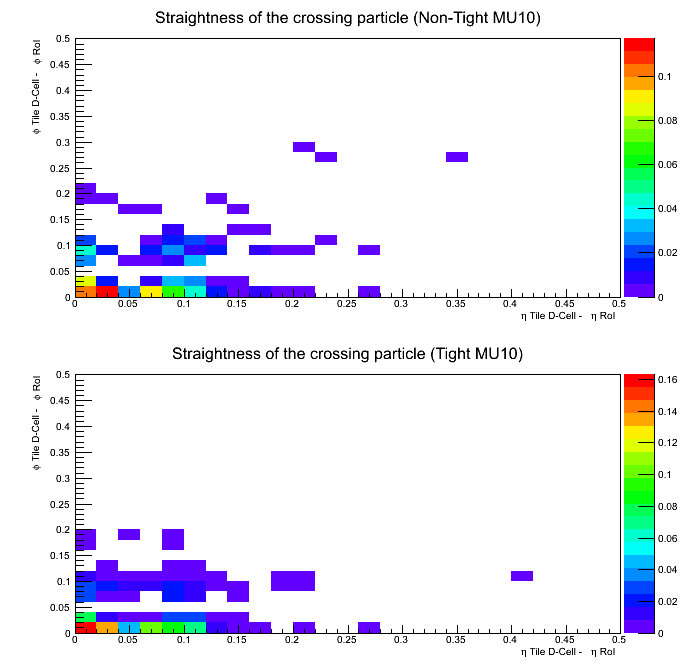
\includegraphics[width=11cm]{images/minbias/crossGeo.png}
    \caption{Histograma apresentando o quão oblíqua é a trajetória do múon. O
    primeiro gráfico representa os eventos com partículas não confirmadas pelo
    critério \emph{tight}, enquanto no segundo apenas confirmadas.}
    \label{crossgeominbias}
\end{figure}

\begin{figure}[htpb!]
        \centering
        \begin{subfigure}[b]{0.45\textwidth}
                \centering
                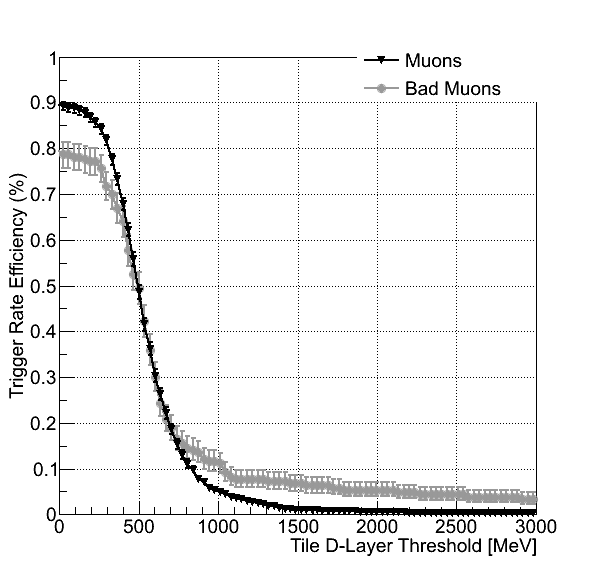
\includegraphics[width=\textwidth]{images/minbias/C_match.png}
        \end{subfigure}%
        ~
        \begin{subfigure}[b]{0.45\textwidth}
                \centering
                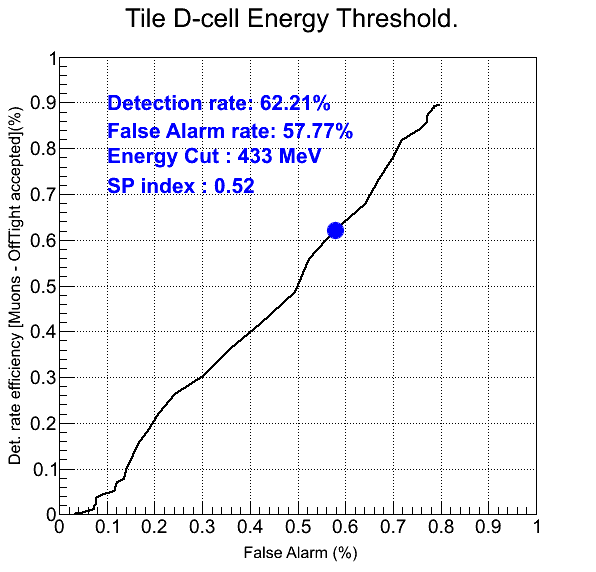
\includegraphics[width=\textwidth]{images/minbias/C_roc_match.png}
        \end{subfigure}
        \caption{Curva ROC para o uso de patamar de energia ao casar as
        geometrias do TileCal e do RPC.}
        \label{fig:ROCSLminbias}
\end{figure}


\subsection*{Discriminador Neural}

Foi novamente escolhida a metodologia de validação cruzada para o projeto do
discriminador neural. Primeiramente, as amostras foram agrupadas em 9
\emph{clusters}. O número de \emph{clusters} utilizado foi determinado pelo
índice de Davies-Bouldin. A Figura~\ref{fig:clustersminbias} mostra o resultado da
divisão em agrupamentos. Mais uma vez, nenhum dos \emph{clusters} formados
evidenciou uma das classes.

\begin{figure}[htpb!]
    \centering
    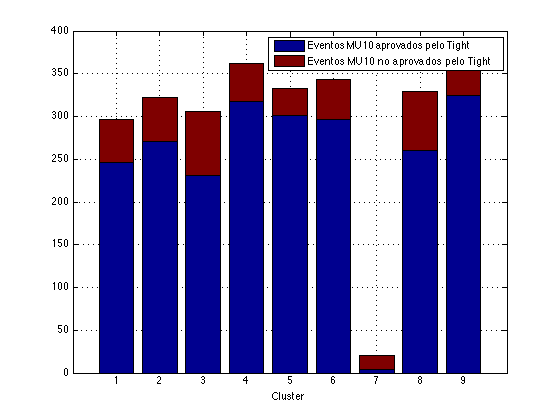
\includegraphics[width=11cm]{images/minbias/kmeans_cluster.png}
    \caption{Eventos de múon separados em 9 \emph{clusters} depois de aplicado
    o algoritmo de \emph{K-means}.}
    \label{fig:clustersminbias}
\end{figure}

Os dados dos \emph{clusters} foram igualmente distribuídos entre 10 os blocos.
As Figuras~\ref{fig:blocominbias-1}, \ref{fig:blocominbias-2} e
\ref{fig:blocominbias-3} mostram os dados distribuídos nos blocos. Neste ponto,
as informações sobre múons falsos são replicadas em cada um dos blocos, de forma
que a representatividade das duas classes seja parelha.


\begin{sidewaysfigure}
    \centering
    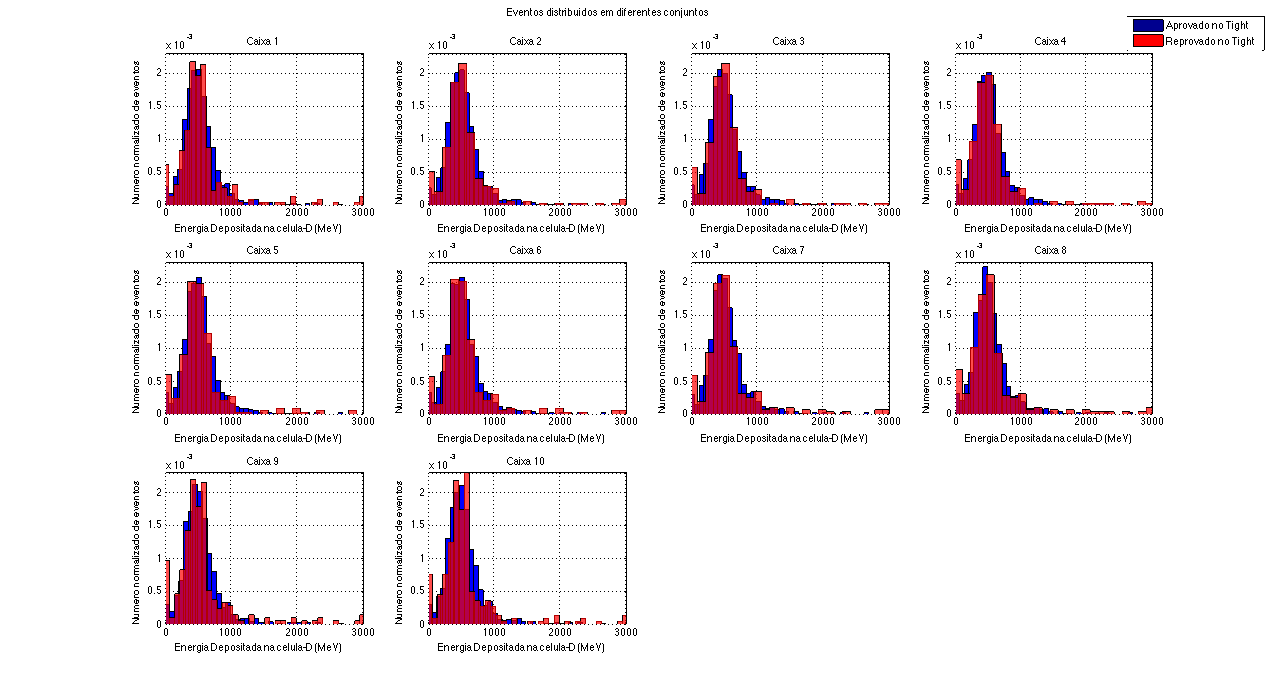
\includegraphics[width=\textheight]{images/minbias/histClusters.png}
    \caption{Eventos de múons divididos em 10 blocos. As distribuições da
    energia depositada na célula D. Os histogramas dos diferentes blocos devem
    ser semelhantes.}
    \label{fig:blocominbias-1}
\end{sidewaysfigure}

\begin{sidewaysfigure}
    \centering
    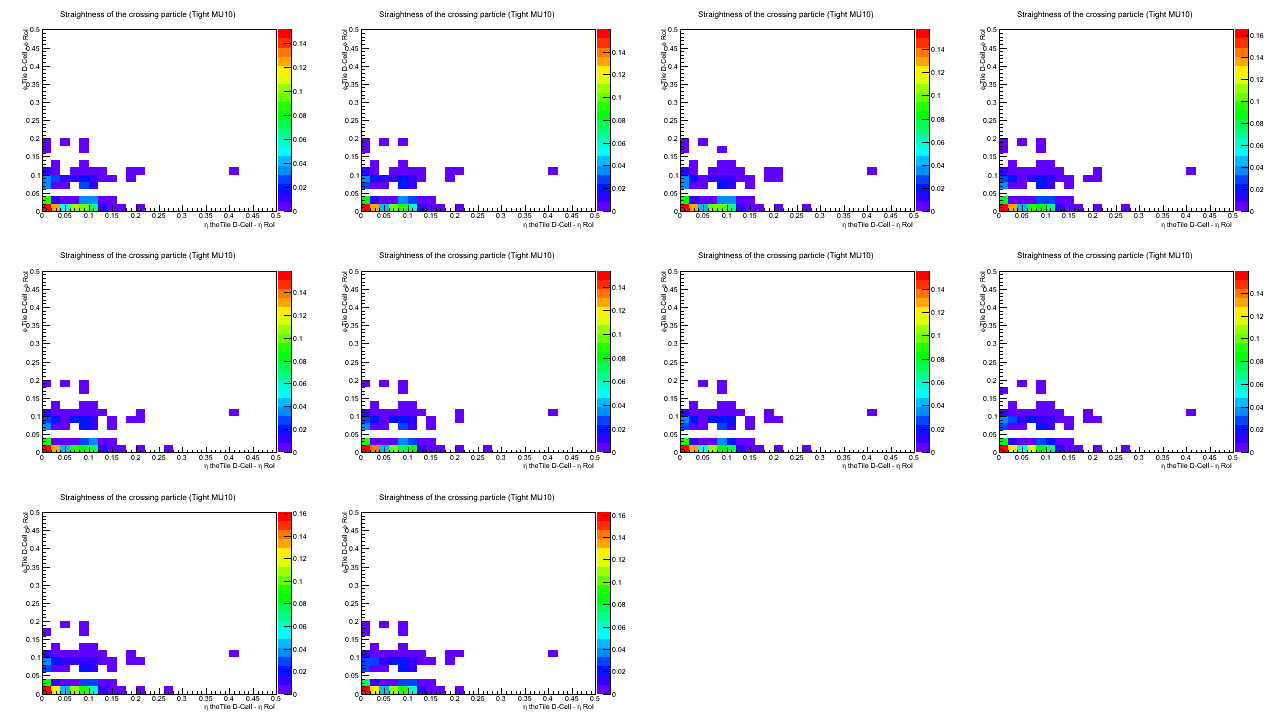
\includegraphics[width=\textheight]{images/minbias/cluster_phi_eta_class.png}
    \caption{Eventos de múons divididos em 10 blocos. \emph{Hits} na camada D do
    TileCal e nas regiões de interesse do RPC. Todos eventos aprovados pelo
    critério \emph{tight}.}
    \label{fig:blocominbias-2}
\end{sidewaysfigure}

\begin{sidewaysfigure}
    \centering
    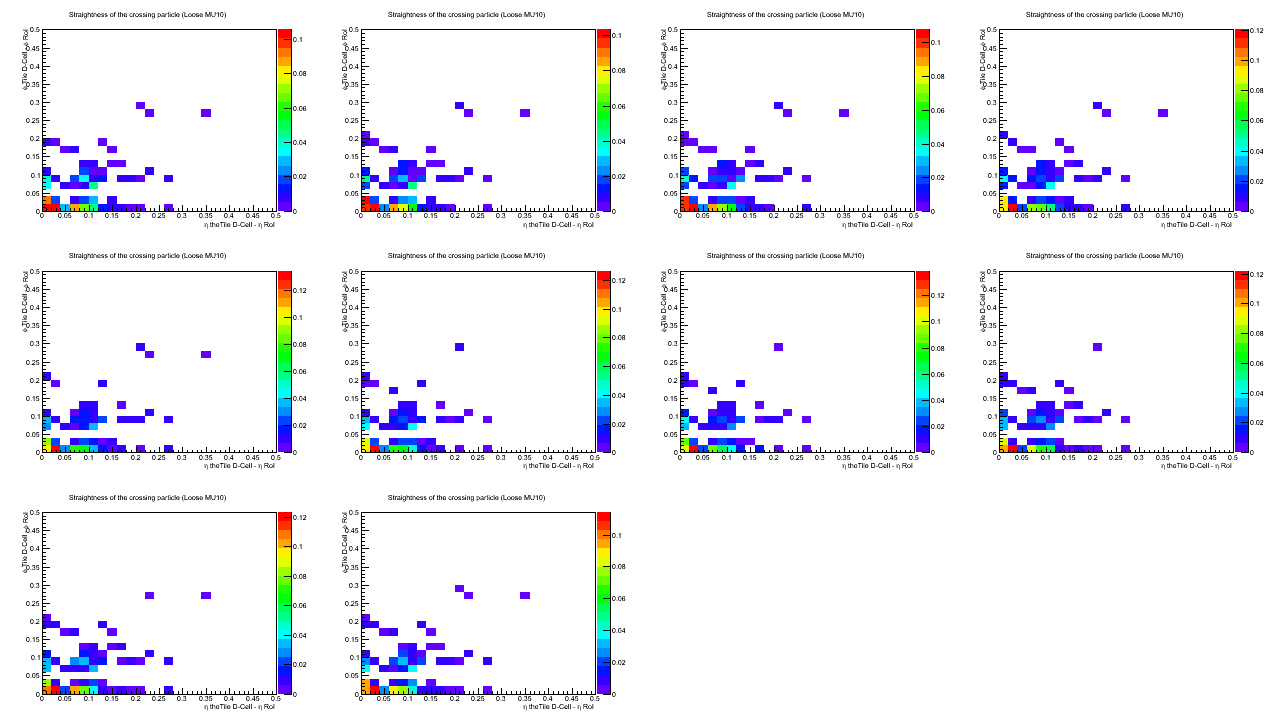
\includegraphics[width=\textheight]{images/minbias/cluster_phi_eta_noclass.png}
    \caption{Eventos de múons divididos em 10 blocos. \emph{Hits} na camada D do
    TileCal e nas regiões de interesse do RPC. Todos eventos reprovados pelo
    critério \emph{tight}.}
    \label{fig:blocominbias-3}
\end{sidewaysfigure}

Ao todo, 30 topologias foram treinadas. Por sua vez, cada uma foi treinada com
10 arranjos diferentes de treino, teste e validação. Cada rede foi inicializada
20 vezes com intuito de evitar mínimos locais e a que tiver melhor índice de SP
para o conjunto de validação será armazenada. No total, foram realizadas 6.000
rodadas de treino para selecionar a topologia ideal.

A Figura~\ref{fig:Topologyminbias} mostra o índice de SP médio para cada
topologia treinada, levando em consideração os 10 blocos utilizados. No gráfico,
ainda é possível verificar o valor máximo e mínimo conseguido. A incerteza é
representada pelo desvio padrão. Levando em consideração o SP mais elevado, a
rede com 29 neurônios na camada escondida foi escolhida.

A Figura~\ref{fig:ROCNNminbias} apresenta a  curva ROC para a rede com 29
neurônios na camada intermediária que obteve maior valor SP para o conjunto de
validação de dados. Neste caso, observou-se um grande aumento de performance. A
taxa de detecção aumenta cerca de 20\% em relação aos outros métodos utilizados
e o falso-alarme é reduzido a 40\%.

\begin{figure}[htpb!]
    \centering
        \begin{subfigure}[b]{0.45\textwidth}
                \centering
            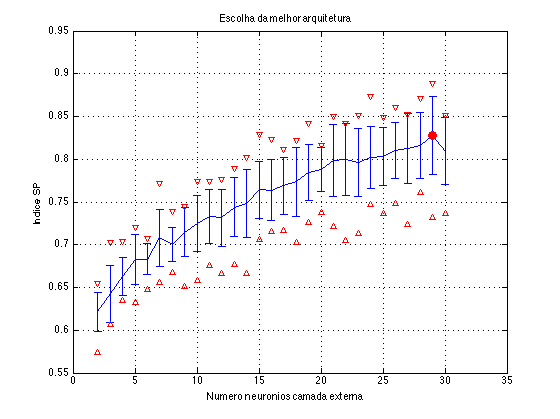
\includegraphics[width=\textwidth]{images/minbias/plotSP.png}
            \caption{Escolha da melhor Topologia. Com base nesse gráfico podemos
            perceber que a topologia com 29 neurônios na camada oculta obteve
            melhor desempenho.}
            \label{fig:Topologyminbias}
        \end{subfigure}%
        ~
        \begin{subfigure}[b]{0.45\textwidth}
                \centering
                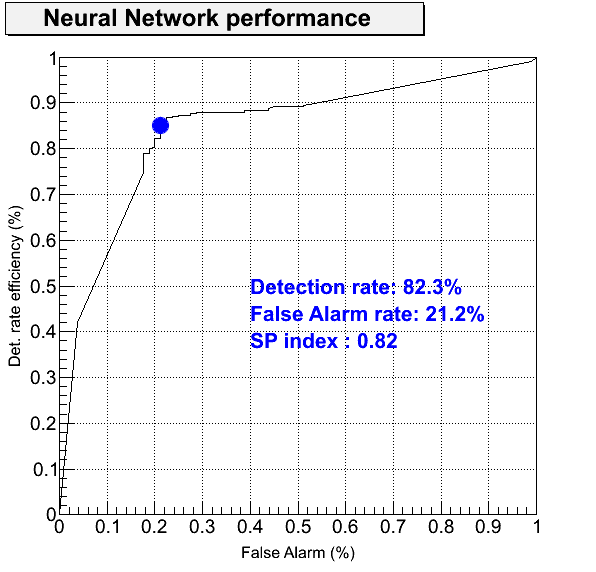
\includegraphics[width=\textwidth]{images/minbias/C_roc_nn.png}
            \caption{Curva ROC para saída da rede neural com 29 neurônios na
            camada oculta.}
            \label{fig:ROCNNminbias}
        \end{subfigure}
        \caption{Projeto de discriminador neural.}
\end{figure}

